\documentclass{report}

\usepackage{hyperref}

\usepackage{epstopdf}
\usepackage{amsmath}
\usepackage{amssymb}
\usepackage{subfig}
%\usepackage{multirow}
\usepackage[utf8]{inputenc}
\usepackage[T1]{fontenc}
\usepackage{standalone}
\usepackage{tikz}
\usepackage{tabularx}
\usepackage{float}
\usepackage[section]{placeins}
\usepackage{sverb}
\usepackage{import}
\usepackage{verbatim}
\usepackage{listings}
\usepackage{xcolor}

\graphicspath{{img/}}
\DeclareGraphicsExtensions{.pdf,.png,.jpg,.svg} %For pdflatex






\definecolor{codegreen}{rgb}{0,0.6,0}
\definecolor{codegray}{rgb}{0.5,0.5,0.5}
\definecolor{codepurple}{rgb}{0.58,0,0.82}
\definecolor{backcolour}{rgb}{0.95,0.95,0.92}

\lstdefinestyle{mystyle}{
    backgroundcolor=\color{backcolour},   
    commentstyle=\color{codegreen},
    keywordstyle=\color{magenta},
    numberstyle=\tiny\color{codegray},
    stringstyle=\color{codepurple},
    basicstyle=\ttfamily\footnotesize,
    breakatwhitespace=false,         
    breaklines=true,                 
    captionpos=b,                    
    keepspaces=true,                 
    numbers=left,                    
    numbersep=5pt,                  
    showspaces=false,                
    showstringspaces=false,
    showtabs=false,                  
    tabsize=2,
    float=H,
    extendedchars=\true, 
}


\lstset{style=mystyle}


\begin{document}

\begin{titlepage}
    \begin{center}
        
\includegraphics[width=.50\linewidth]{other/polsl.png}\\
        \Huge
        \textbf{Przetwarzanie Obrazów Cyfrowych}
        \\ \vspace{1.5cm}
        \Large
        \textbf{Raport z ćwiczenia nr. 6: } \\
        % \textbf{WSTĘPNE PRZETWARZANIE OBRAZÓW — FILTRY LINIOWE}
        \textbf{Wstępne przetwarzanie obrazów - filtry liniowe}        
    \end{center}
    \vspace{3.0cm}
    \Large
    Raport opracował: \\
    Dawid Kania \\
    Grupa 6 Semestr 6 \\ \\
    Data wykonania ćwiczenia: 09.06.2022
\end{titlepage}
 


\section*{Zadanie 1}

\newcommand{\ww}{0.32333} 
\begin{figure}[H] 
    \captionsetup[subfloat]{justification=raggedright,singlelinecheck=false, position=bottom,labelformat=empty} % 
    \subfloat[Wielkość obrazu O1: 500x512]{
       
\includegraphics[width=\ww\linewidth]{../zad1/img1/O1___.png}}  \hfill% 
    \subfloat[Wielkość obrazu: 500x512\\ Wielkość maski: 3x3]{
       
\includegraphics[width=\ww\linewidth]{../zad1/img1/O1_Md.png}}  \hfill% 
    \subfloat[Wielkość obrazu: 500x512\\ Wielkość maski: 3x3]{
       
\includegraphics[width=\ww\linewidth]{../zad1/img1/O1_Mg.png}}  \\ 
    \subfloat[Wielkość obrazu O1: 500x512]{
       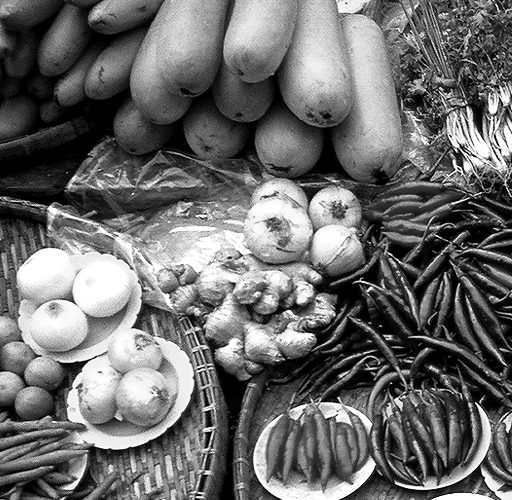
\includegraphics[width=\ww\linewidth]{../zad1/img4/O1___.png}}  \hfill% 
    \subfloat[Wielkość obrazu: 500x512\\ Wielkość maski: 3x3]{
       
\includegraphics[width=\ww\linewidth]{../zad1/img4/O1_Md.png}}  \hfill% 
    \subfloat[Wielkość obrazu: 500x512\\ Wielkość maski: 3x3]{
       
\includegraphics[width=\ww\linewidth]{../zad1/img4/O1_Mg.png}}
\caption{Porownanie}  
\label{fig:../zad1/result_1_4.tex} 
\end{figure} 
\let\ww\undefined 
maski użyte do filtracji obrazu:
$$
\begin{array}{cc}
Md =  \begin{bmatrix}  \frac{1}{9} & \frac{1}{9} & \frac{1}{9}\\[6pt]
 \frac{1}{9} & \frac{1}{9} & \frac{1}{9}\\[6pt]
 \frac{1}{9} & \frac{1}{9} & \frac{1}{9} \end{bmatrix} 
&
Mg =  \begin{bmatrix}  0 & -1 & 0\\[6pt]
 -1 & 4 & -1\\[6pt]
 0 & -1 & 0 \end{bmatrix} 
\end{array}
$$
\newcommand{\ww}{0.32333} 
\begin{figure}[H] 
    \captionsetup[subfloat]{justification=raggedright,singlelinecheck=false, position=bottom,labelformat=empty} % 
    \subfloat[Wielkość obrazu O1: 500x512]{
       
\includegraphics[width=\ww\linewidth]{../zad1/img2/O1___.png}}  \hfill% 
    \subfloat[Wielkość obrazu: 500x512\\ Wielkość maski: 3x 3x]{
       
\includegraphics[width=\ww\linewidth]{../zad1/img2/O1_Md.png}}  \hfill% 
    \subfloat[Wielkość obrazu: 500x512\\ Wielkość maski: 3x 3x]{
       
\includegraphics[width=\ww\linewidth]{../zad1/img2/O1_Mg.png}}  \\ 
    \subfloat[Wielkość obrazu O1: 500x512]{
       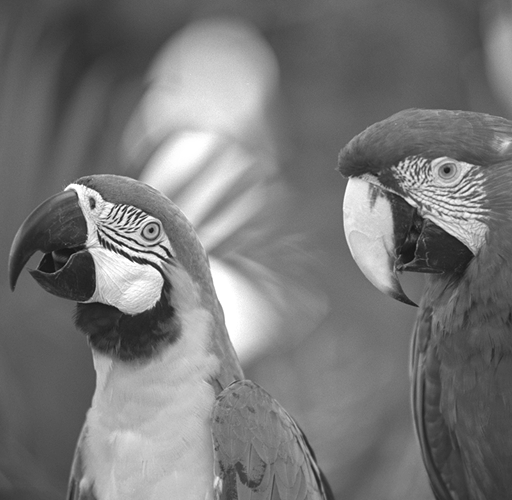
\includegraphics[width=\ww\linewidth]{../zad1/img5/O1___.png}}  \hfill% 
    \subfloat[Wielkość obrazu: 500x512\\ Wielkość maski: 3x 3x]{
       
\includegraphics[width=\ww\linewidth]{../zad1/img5/O1_Md.png}}  \hfill% 
    \subfloat[Wielkość obrazu: 500x512\\ Wielkość maski: 3x 3x]{
       
\includegraphics[width=\ww\linewidth]{../zad1/img5/O1_Mg.png}}
\caption{Porownanie}  
\label{fig:../zad1/result_2_5.tex} 
\end{figure} 
\let\ww\undefined 
maski użyte do filtracji obrazu:
$$
\begin{array}{cc}
Md =  \begin{bmatrix}  \frac{1}{9} & \frac{1}{9} & \frac{1}{9}\\[6pt]
 \frac{1}{9} & \frac{1}{9} & \frac{1}{9}\\[6pt]
 \frac{1}{9} & \frac{1}{9} & \frac{1}{9} \end{bmatrix} 
&
Mg =  \begin{bmatrix}  0 & -1 & 0\\[6pt]
 -1 & 4 & -1\\[6pt]
 0 & -1 & 0 \end{bmatrix} 
\end{array}
$$
\newcommand{\ww}{0.32333} 
\begin{figure}[H] 
    \captionsetup[subfloat]{justification=raggedright,singlelinecheck=false, position=bottom,labelformat=empty} % 
    \subfloat[Wielkość obrazu O1: 500x512]{
       
\includegraphics[width=\ww\linewidth]{../zad1/img3/O1___.png}}  \hfill% 
    \subfloat[Wielkość obrazu: 500x512\\ Wielkość maski: 3x 3x]{
       
\includegraphics[width=\ww\linewidth]{../zad1/img3/O1_Md.png}}  \hfill% 
    \subfloat[Wielkość obrazu: 500x512\\ Wielkość maski: 3x 3x]{
       
\includegraphics[width=\ww\linewidth]{../zad1/img3/O1_Mg.png}}  \\ 
    \subfloat[Wielkość obrazu O1: 500x512]{
       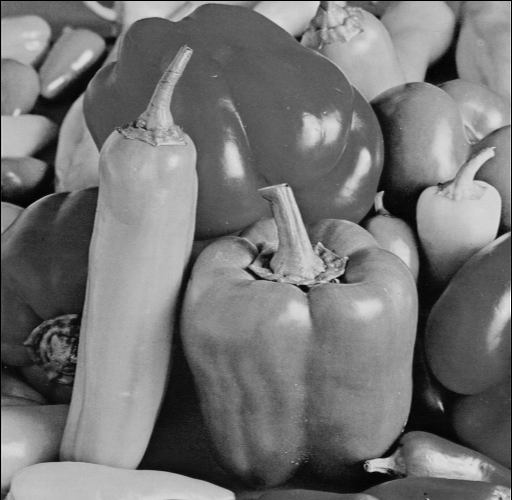
\includegraphics[width=\ww\linewidth]{../zad1/img6/O1___.png}}  \hfill% 
    \subfloat[Wielkość obrazu: 500x512\\ Wielkość maski: 3x 3x]{
       
\includegraphics[width=\ww\linewidth]{../zad1/img6/O1_Md.png}}  \hfill% 
    \subfloat[Wielkość obrazu: 500x512\\ Wielkość maski: 3x 3x]{
       
\includegraphics[width=\ww\linewidth]{../zad1/img6/O1_Mg.png}}
\caption{Porownanie}  
\label{fig:../zad1/result_3_6.tex} 
\end{figure} 
\let\ww\undefined 
maski użyte do filtracji obrazu:
$$
\begin{array}{cc}
Md =  \begin{bmatrix}  \frac{1}{9} & \frac{1}{9} & \frac{1}{9}\\[6pt]
 \frac{1}{9} & \frac{1}{9} & \frac{1}{9}\\[6pt]
 \frac{1}{9} & \frac{1}{9} & \frac{1}{9} \end{bmatrix} 
&
Mg =  \begin{bmatrix}  0 & -1 & 0\\[6pt]
 -1 & 4 & -1\\[6pt]
 0 & -1 & 0 \end{bmatrix} 
\end{array}
$$


\section*{Zadanie 2}



% \newpage \section*{Kody programów}
% \subsection*{ zad1.m                }  \lstinputlisting[language=Octave]{ ../matlab/zad1.m                } \newpage
% \subsection*{ zad2.m                }  \lstinputlisting[language=Octave]{ ../matlab/zad2.m                } \newpage





\end{document}